\subsection{Introduction}

  \lettrine[nindent=0em,lines=3]{L} es systèmes multicoeurs modernes sont
  maintenant basés sur l'architecture NUMA (Non Uniforme Memory Access). Avec un
  système NUMA, les coeurs des processeurs sont regroupés en noeuds. Chaque
  noeud possède un contrôleur mémoire et est interconnecté avec les autres
  noeuds de la machine.

  \begin{figure}[H]
    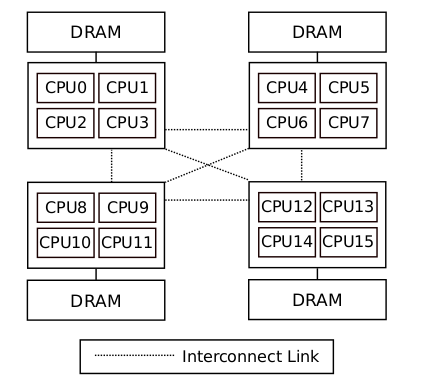
\includegraphics[scale=0.4]{img/numa_arch.png}
    \caption{Un système NUMA avec 4 noeuds et 4 coeurs par noeud}
    \label{f:numa_arch}
  \end{figure}

  Du fait des temps d'accès mémoire non uniforme, tout le défi des systèmes
  tournant sur cette architecture est la répartition des données et des
  traitements. En effet, la principale cause de latence n'est pas due au
  \textbf{temps de traitement des données}, mais au \textbf{temps d'accès aux
    données}. Ces accès coûtent entre 10\% et 40\% de temps supplémentaire par
  rapport aux accès locaux.\cite{Lepers2014} Dans une configuration idéale,
  chaque coeur irait chercher ce dont il a besoin dans la mémoire contrôlée par
  le noeud dans lequel il se situe. Ainsi, les demandes d'accès distant seraient
  réduites à néant, et il n'y aurait aucune latence due aux échanges entre les
  noeuds. Nous allons voir que cet idéal est très difficile, voire impossible à
  obtenir. Néanmoins, il est possible de s'en approcher, en mettant au point des
  algorithmes de répartitions de plus en plus efficaces. La création de ces
  algorithmes nécessite une connaissance approfondie du noyau: comment gère-t-il
  la création des threads, où sont-ils placés, quelles sont les pages mémoires
  accédées le plus souvent, par quels noeuds sont-elles contrôlées\ldots C'est
  en collectant un maximum de renseignements sur ces différents points (et de
  nombreux autres) que l'on pourra être en mesure d'affiner les solutions de
  répartition de charge. Cette étape de monitoring sera le sujet principal de ce
  projet de master. Nous allons devoir lire et comprendre le fonctionnement à
  très bas niveau du noyau, puis le modifier en utilisant divers outils de
  gestions d'évènements avec des bibliothèques comme IBS\footnote{Instruction
    Base Samplign, une technologie développée par AMD uniquement sur les
    processeurs Opteron} afin de préparer l'étape de réflexion pour la création
  d'algorithmes.
